\documentclass[12pt,fleqn]{examtst}
\usepackage{graphicx}
\usepackage{amssymb}
\usepackage{amsmath}
\usepackage{listings}
\usepackage{multirow}
\usepackage{multicol}
\usepackage{hhline}
\usepackage{booktabs}
\usepackage{url}
\usepackage{enumerate}
\usepackage{hyperref}
%% Comments

\usepackage{color}

\newif\ifcomments\commentstrue

\ifcomments
\newcommand{\authornote}[3]{\textcolor{#1}{[#3 ---#2]}}
\newcommand{\todo}[1]{\textcolor{red}{[TODO: #1]}}
\else
\newcommand{\authornote}[3]{}
\newcommand{\todo}[1]{}
\fi

\newcommand{\wss}[1]{\authornote{blue}{SS}{#1}}

\begin{document}

\newcommand{\soln}{n} %y for yes and n for no

\lstset{language=python, basicstyle=\ttfamily, breaklines=true,
  showspaces=false, showstringspaces=false, breakatwhitespace=true, texcl=true,
  escapeinside={\%*}{*)}}

\newcommand{\codeit}[1]{\texttt{\textit{#1}}}

\begin{center}
  {\large \bf COMP SCI 2ME3 and SFWR ENG 2AA4 Final Examination}\\[1ex]
  {\large \bf McMaster University}\\[1ex]
  \ifthenelse{\equal{\soln}{y}}{\large {\bf Answer Key:} Large arrow
    ($\Longleftarrow$) for correct% , small ($\leftarrow$) for partially
    % correct
  }{}
\end{center}

\medskip

\noindent
DAY CLASS, \textbf{Version 1}  \hfill Dr.~S.~Smith \\
DURATION OF EXAMINATION: 2.5 hours (+ 30 minutes buffer time)\\
MCMASTER UNIVERSITY FINAL EXAMINATION \hfill April 28, 2021

\medskip

\noindent
\rule[3 mm]{\textwidth}{0.5mm}

%\begin{minipage}[t]{1.0\textwidth}

NAME: \wss{Enter your name here}\\[1ex]

Student ID: \wss{Enter your student number here} \\[2mm]

\noindent
\rule[3 mm]{\textwidth}{0.5mm}

This examination paper includes \noofpages pages and
8 % VARIABILITY
questions. You are responsible for ensuring that your copy of the examination
paper is complete. Bring any discrepancy to the attention
of your instructor.\\

\noindent
\emph{By submitting this work, I certify that the work represents solely my own
independent efforts. I confirm that I am expected to exhibit honesty and use
ethical behaviour in all aspects of the learning process.  I confirm that it is
my responsibility to understand what constitutes academic dishonesty under the
\href{https://secretariat.mcmaster.ca/app/uploads/Academic-Integrity-Policy-1-1.pdf}
{Academic Integrity Policy}}.\\

\noindent
\textbf{Special Instructions}:

\begin{enumerate}

\item For taking tests remotely: 
\begin{itemize}
\item Turn off all unnecessary programs, especially Netflix, YouTube, games like
  Xbox or PS4, anything that might be downloading or streaming.
\item If your house is shared, ask others to refrain from doing those activities
  during the test.
\item If you can, connect to the internet via a wired connection.
\item Move close to the Wi-Fi hub in your house. 
\item Restart your computer, 1-2 hours before the exam. A restart can be very
  helpful for several computer hiccups.
\item Use a VPN (Virtual Private Network) since this improves the connection to
  the CAS servers.
\item Commit and push your tex file, compiled pdf file, and code files
  frequently.  As a minimum you should do a commit and push after completing
  each question.
\item Ensure that you push your solution (tex file, pdf file and code files)
  before time expires on the test.  The solution that is in the repo at the
  deadline is the solution that will be graded.
\item If you have trouble with your git repo, the quickest solution may be to
  create a fresh clone.
\end{itemize}
\item It is your responsibility to ensure that the answer sheet is properly
  completed. Your examination result depends upon proper attention to the
  instructions.
\item All physical external resources are permitted, including textbooks, calculators,
  computers, compilers, and the internet.
\item The work has to be completed individually.  Discussion with others is
  strictly prohibited.
\item Read each question carefully.
\item Try to allocate your time sensibly and divide it appropriately between the
  questions.  Use the allocated marks as a guide on how to divide your time
  between questions.
\item The quality of written answers will be considered during grading.  Please
  make your answers well-written and succinct.
\item The set $\mathbb{N}$ is assumed to include $0$.
\end{enumerate}
%\end{minipage}\\

\examheader{CS2ME3/SE2AA4 \ifthenelse{\equal{\soln}{y}} {\hfill SOLUTIONS} }

\renewcommand{\labelenumi}{\Alph{enumi}.}

\newpage

%%%%%%%%%%%%%%%%%%%%%%%%%%%%%%%%%%%%%%%%%%%%%%%%%%%%%%%%%%%%%%%%%%%%%%

\question{5 marks} What are the problems with using ``average lines of code
written per day'' as a metric for programmer productivity?

\bigskip

\noindent \wss{Provide your reasons in the itemized list below.  Add more items
  as required.}

\begin{itemize}
\item This is quite a novice mistake; it is important to realize that a longer code does not always mean a better code. Succinct code is oftentimes far more advantageous in many areas. If the programmer practices incremental testing, as is best, by the time they finish their code they might end up with far more than necessary test cases. Having more test cases also does not mean that the testing process was more efficient; they may fail to test boundary cases. With succinct code, the programmer is given the ability to better decide on important testing cases such as boundaries. In addition, longer codes risk cluttering, making it harder to read and to understand by another developer, on top of making the debugging process much more of a hassle, should they fail to incrementally verify their program. They risk affecting major software qualities such as generality, minimality, and essentiality by overdoing what may be required for a simple method. By overdoing code, they may in turn add too many specifics such that the program cannot reusable in the long term. Furthermore, maintainability is affected in that there is much more to go over every time a change needs to be made. These in turn risk failing to meet the software requirements. It is best to judge programmer productivity through incremental testing, ensuring that whatever they have is correct, and not by the average amount of lines. Writing more code is a waste of resources and time that could be better spent on important program qualities to complete. 

\end{itemize}

%%%%%%%%%%%%%%%%%%%%%%%%%%%%%%%%%%%%%%%%%%%%%%%%%%%%%%%%%%%%%%%%%%%%%%

\newpage

\question{5 marks} Critique the following requirements specification
for a new cell phone application, called CellApp.  Use the following criteria
discussed in class for judging the quality of the specification: abstract,
unambiguous, and validatable.  How could you improve the requirements
specification?

\bigskip

``The user shall find CellApp easy to use.''

\bigskip

\noindent \wss{Fill in the itemized list below with your answers.  Leave the
  word in bold at the beginning of each item.}

\begin{itemize}
\item \textbf{Abstract} - This specification is abstract in that it tells the developer the "what" such that the program should be easy to use, however it does not tell the developer the "how". By not providing the "how", the specification leaves an open opportunity to for the developer to go about "making the CellApp easy to use" in a way that they feel fit. Based on the full abstraction, however, the developer is left to make assumptions which leads to ambiguity as discussed in the next point. 
\item \textbf{Unambiguous} - The terms "easy to use" or "user friendly" as extremely ambiguous. The developer does not know who the target user is, they may come from a different age range, technical background, etc. It is very subjective to say user friendly; what may be easy to use for one person can be difficult to use by another. 
\item \textbf{Validatable} - Tying closely to ambiguity, it is difficult to measure validability of this specification. By the subjectivity of the specification, the developer may find it difficult to test or measure success and failure in meeting the requirement. It is hard to quantify "easy" without specific requirements. The ambiguity of this specification leads to misunderstanding between the developer and the client, such that even though the developer may find it user-friendly, the client may not and for this reason a viable test cannot take place to validate the requirement. 
\item \textbf{How to improve} - There are ways to improve this specification, by clearly identifying what the client considers "user-friendly". Extend the context by requiring, perhaps, "a certain amount of clicks made by the user", or testing by implementing surveys for user feedback. In doing so, the developer and client may come to a clearer agreement and the developer is one step closer to ensuring that they are making the right product
\end{itemize}

%%%%%%%%%%%%%%%%%%%%%%%%%%%%%%%%%%

\newpage

\question{5 marks} The following module is proposed for the maze tracing robot
we discussed in class (L20).  This module is a leaf module in the decomposition
by secrets hierarchy.

\begin{description}
\item [Module Name] find\_path
\item [Module Secret] The data structure and algorithm for finding the shortest
  path in a graph.
\end{description}

\noindent \wss{Fill in the answers to the questions below.  For each item you
  should leave the bold question and write your answer directly after it.}

\begin{enumerate}
\item \textbf{Is this module Hardware Hiding, Software Decision Hiding or
    Behaviour Hiding?  Why?}

  - This module falls under Software Decision Hiding. Noting that the software requirements specification (SRS) is abstract, the developer becomes more concrete in the Module Guide, then more concrete in the MIS, and then even more concrete in the actual code. Decisions, such as determining the algorithm and data structure for the shortest path, fall under the category of Software Decision hiding in that it makes the service less abstract. Modules such as this provide generic services that can be used elsewhere if need be. Services such as this, solve the ODE. 

\item \textbf{Is this a good secret?  Why?}

  - This is not a good secret. The secret uses nouns such as "data structure" and "algorithm" which is efficient, but it fails to adhere to having one secret for one module. By using "and", the secret suggests that the module implements both the data structure and algorithm for finding the shortest path, leaving it two responsibilities. It would be better to split this into two modules; one for the data structure for finding the shortest path, and one for the algorithm for finding the shortest path. By having too many secrets, the module risks not being cohesive.  

\item \textbf{Does the specification for maze tracing robot require environment
    variables?  If so, which environment variables are needed?}

  - The developer should implement environment variables such as the display or the screen available to the user, along with the position (cell) at which the pen or tracker is currently on. We should additionally implement environment variables to recognize the state of the game, i.e. new game, lost game, or completed path, etc.

\end{enumerate}

%%%%%%%%%%%%%%%%%%%%%%%%%%%%%%%%%%

\newpage

\question{5 marks} Answer the following questions assuming that you are in doing
your final year capstone in a group of 5 students.  Your project is to write a
video game for playing chess, either over the network between two human
opponents, or locally between a human and an Artificial Intelligence (AI)
opponent.

\bigskip

\noindent \wss{Fill in the answers to the questions below.  For each item you
  should leave the bold question and write your answer directly after it.}

\begin{enumerate}
  
\item \textbf{You have 8 months to work on the project.  Keeping in mind that we
  usually need to fake a rational design process, what major milestones and what
  timeline for achieving these milestones do you propose?  You can indicate the
  time a milestone is reached by the number of months from the project's start date.}

  - At the beginning of the 8 months, we are given an abstract problem statement. It is critical to begin the rational design process immediately. The development plan and requirements should take a month to complete, giving us time to carefully create possible test cases and determine what needs to get done to meet the client needs. Over the span of the second to the third month, we should have completed sketches and ultimate rough draft or the module guides and MIS in order to begin the implementation. I assume the implementation of the code, as it becomes less abstract, will take the majority of our time. From month 3 to month 6 or month 7, we should be working on coding and incrementally testing as we go in order to avoid last minute defects and stress. We should be verifying everything as we go, in addition to noting and observing likely changes and making changes accordingly. We must ensure to test as many possbilities as we can. By the last one to two months (month 7 to month 8), we should be stress testing and ensuring that our project is compatible, portable and ready to be used for the presentation and by other users.   
  
\item \textbf{Everything in your process should be verified, including the
    verification.  How might you verify your verification?}

  - Mutant testing is a feasible method of verifying the verification. By using employing the "Potato Lake" method, this artifical seeding of faults aids in discovering both seeded and new faults, which is used to estimate the total number of errors or faults in the code. Through this, we can grasp and assume that the proability of errors (total) is proportional to the number of errors already found with respect to the whole program. Mutation testing can be done by generating simple changes to the source code, which become faults. This can be done by modifying operations and constants or by changing the order of certain executions. It is not guaranteed that all of these modifications will produce an error, but it is safe to assume the majority of them will. We can ultimately establish the adequacy of our Test Set from from running our tests on each of our generate faults (mutants).
  
\item \textbf{How do you propose verifying the installability of your game?}

  - Given that there are variations in operating systems, there are multiples risks in not verifying installability, especially towards the end of the project. If for example the project runs on the developer's Mac OS for example, they must also ensure to, throughout the entire development process (8 months), ensure that someone is able to run it on Microsoft or any other operating system as well. Failing to do so will result in possible major risks in the final presentation of our software. Another way to verify installability, if for example academic integrity is a concern, is through the use of a Virtual Machine. 
  
\end{enumerate}

%%%%%%%%%%%%%%%%%%%%%%%%%%%%%%%%%%%%%%%%%%%%%%%%%%%%%%%%%%%%%%%%%%%%%%

\newpage

\question{5 marks} As for the previous question, assume you are doing a final
year capstone project in a group of 5 students.  As above, your project
is to write a video game for playing chess, either over the network between two
human opponents, or locally between a human and an Artificial Intelligence
(AI) opponent.  The questions below focus on verification and testing.

\bigskip

\noindent \wss{Fill in the answers to the questions below.  For each item you
  should leave the bold question and right your answer directly after it.}

\begin{enumerate}
\item \textbf{Assume you have 4 work weeks (a work week is 5 days) over the
    course of the project for verification activities.  How many collective
    hours do you estimate that your team has available for verification related
    activities?  Please justify your answer.}

  - My group and I are presumably enrolled in other courses, meaning we cannot work on this project as much as we'd like to (i.e. full time :)). Based on this, a realistic amount of hours a week on testing would be 10 hours, approximately 2 hours a day for a 5 day week(if not less). Towards the end, I assume the emphasis for verfication will increase significantly. The amount of verification within four weeks should be amplified as opposed to the amount of verification within an 8 month span. In total, the collective hours spent of verification would be just below 40 hours, be that dynamic or static. 
  
\item \textbf{Given the estimated hours available for verification, what verification
    techniques do you recommend for your team?  Please list the techniques,
    along with the number of hours your team will spend on each technique, and
    the reason for selecting this technique.}

  - The best method is to incrementally verify our project, in terms of installability, working codes through unit testing. We should implement both dynamic as static testing. Through incremental testing, dynamic testing should not be too much of a stress; we test the behaviour of our code as we go through white-box and black-box testing. In terms of static analysis, it is best that we gather and ask specific questions pertaining to our documentation, i.e. "will this loop ever run", "is the syntax correct", "is this specification ambiguous/essential, etc". Given that we have our peers (not in capstone due to academic integrity) and group members as an available resource, we should take advanatge of periodic code walkthroughs, inspections, and most practically on our own time, rubber duck testing to ensure that what we are creating realyl and truly makes sense.
  
\item \textbf{Is the oracle problem a concern for implementing your game?  Why
    or why not?  If it is a concern, how do you recommend testing your software?}

  - Since oracles are requires at each stage of testing, are quite difficult to design \textit{and} we only have four weeks, the oracle problem is a concern for implementing our game. We must instead implement strategies without an oracle, such as metamorphism. We can assume a solution, and use it to reversely calculate the inputs that should lead to that solution. We can then use the calculated inputs as inputs again and compare the result to the initially assumed solution. We can use metamorphic relations which specify how changes in our inputs should change the output. We could also use an independent program that can approximate the oracle itself, such as matlab or an already existing game similar to ours, whilst comparing similarities and differences in behaviour.
    
\end{enumerate}

%%%%%%%%%%%%%%%%%%%%%%%%%%%%%%%%%%%%%%%%%%%%%%%%%%%%%%%%%%%%%%%%%%%%%%

\newpage

\question{5 marks} Consider the following natural language specification for a
function that looks for resonance when the input matches an integer multiple of
the wavelengths 5 and 7. Provided an integer input between 1 and 1000, the
function returns a string as specified below:

\begin{itemize}
\item If the number is a multiple of 5, then the output is “resonance 5”
\item If the number is a multiple of 7, then the output is “resonance 7”
\item If the number is a multiple of both 5 and 7, then the output is “resonance
  5 and 7”
\item Otherwise, the output is “no resonance”
\end{itemize}

You can assume that inputs outside of the range 1 to 1000 do not occur.

\begin{enumerate}
\item What are the sets $D_i$ that partition $D$ (the input domain) into a
  reasonable set of equivalence classes?

  We can consider a set of multiples of 5, a set of multiples of 7, a set of multiples of both 5 and 7, and set of neither multiples of 5 nor 7, in which presumably all test lines of code will be considered and tested.

\item Given the sets $D_i$, and the heuristics discussed in class, how would you
  go about selecting test cases?

  It is important to choose values on the specific boundaries, i.e. 5 and 7. In addition we should choose values to test that are quite close to the boundaries, and extremes values, as one would do in the case of black-box testing. In the sense of implementing white-box testing, we would have to take into consideration path coverage (i.e. will we ever get complete path coverage), where we select a test set that traverses all paths from the intiial to the final node of the control flow, if any. We can additionally take into consideration edge coverage (i.e if it is a multiple of 5 and not 7, etc), where we select a test set T such that every edge of the control flow is exercised at least once.
  
\end{enumerate}
  
%%%%%%%%%%%%%%%%%%%%%%%%%%%%%%%%%%

\newpage

\question{5 marks} Below is a partial specification for an MIS for the game of
tic-tac-toe (\url{https://en.wikipedia.org/wiki/Tic-tac-toe}).  You should
complete the specification.

\bigskip

\wss{The parts that you need to fill in are marked by comments, like this one.
  You can use the given local functions to complete the missing specifications.
  You should not have to add any new local functions, but you can if you feel it
  is necessary for your solution.  As you edit the tex source, please leave the
  \texttt{wss} comments in the file.  You can put your answer immediately
  following the comment.}

\subsection* {Syntax}

\subsubsection* {Exported Constants}

SIZE = 3 {\it //size of the board in each direction}\\

\subsubsection* {Exported Types}

cellT = \{ X, O, FREE \} \\

\subsubsection* {Exported Access Programs}

\begin{tabular}{| l | l | l | p{7cm} |}
\hline
\textbf{Routine name} & \textbf{In} & \textbf{Out} & \textbf{Exceptions}\\
\hline
init & ~ & ~ & ~\\
\hline
move & $\mathbb{N}$, $\mathbb{N}$ & ~ & OutOfBoundsException, InvalidMoveException\\
\hline
getb & $\mathbb{N}$, $\mathbb{N}$ & cellT & OutOfBoundsException\\
\hline
get\_turn & ~ & cellT & ~\\
\hline
is\_valid\_move & $\mathbb{N}$, $\mathbb{N}$ & $\mathbb{B}$ & OutOfBoundsException\\
\hline
is\_winner & cellT & $\mathbb{B}$ & ~\\
\hline
is\_game\_over & ~ & $\mathbb{B}$ & ~\\
\hline

\end{tabular}

\subsection* {Semantics}

\subsubsection* {State Variables}

$b$: boardT\\
$\mathit{Xturn}$: $\mathbb{B}$

\subsubsection* {State Invariant}

\wss{Place your state invariant or invariants here}\\
$i > 0 \wedge j > 0$

\subsubsection* {Assumptions}

The init method is called for the abstract object before any other access routine is called for that
object.  The init method can be used to return the state of the game to the state of a new game.

\subsubsection* {Access Routine Semantics}

init():
\begin{itemize}
\item transition: 
$$\mathit{Xturn}, b := \text{true}, 
< \begin{array}{c}
< \mbox{FREE}, \mbox{FREE}, \mbox{FREE} >\\
< \mbox{FREE}, \mbox{FREE}, \mbox{FREE} >\\
< \mbox{FREE}, \mbox{FREE}, \mbox{FREE} >\\
\end{array} >
$$
\item exception: none
\end{itemize}

\noindent move($i$, $j$):
\begin{itemize}
\item transition: $\mathit{Xturn}, b[i, j] := \neg \mathit{Xturn}, (\mathit{Xturn} \Rightarrow \mbox{X} | \neg
\mathit{Xturn} \Rightarrow \mbox{O})$
\item exception
$$exc := (\mbox{InvalidPosition}(i, j) \Rightarrow \mbox{OutOfBoundsException} | \neg \mbox{is\_valid\_move}(i, j)
\Rightarrow \mbox{InvalidMoveException})$$
\end{itemize}

\noindent getb(i, j):
\begin{itemize}
\item output: $\mathit{out} := b[i, j]$
\item exception
$exc := (\mbox{InvalidPosition}(i, j) \Rightarrow \mbox{OutOfBoundsException})$
\end{itemize}

\noindent get\_turn():
\begin{itemize}
\item $output: (\mathit{Xturn} \Rightarrow \mbox{X} | \neg \mathit{Xturn} \Rightarrow \mbox{O})$

\item exception: none
\end{itemize}

\noindent is\_valid\_move(i, j):
\begin{itemize}
\item output: $\mathit{out} := (b[i][j] = \mbox{FREE})$ 
\item exception $exc := (\mbox{InvalidPosition}(i, j) \Rightarrow \mbox{OutOfBoundsException})$
\end{itemize}

\noindent is\_winner(c):
\begin{itemize}
\item output: $\mathit{out} := \mbox{horizontal\_win}(c, b) \vee \mbox{vertical\_win}(c, b) \vee
\mbox{diagonal\_win}(c, b)$ 
\item exception: none
\end{itemize}

\noindent is\_game\_over():
\begin{itemize}
\item output: \wss{Returns true if X or O wins, or if there are no more moves remaining}\\

\item exception: none
\end{itemize}

\subsubsection* {Local Types}

boardT = sequence [SIZE, SIZE] of cellT

\subsubsection* {Local Functions}

\noindent \textbf{InvalidPosition}: $\mathbb{N}$ $\times$ $\mathbb{N}$ $\rightarrow$ $\mathbb{B}$\\
~\newline
InvalidPosition$(i, j) \equiv \neg ( ( 0 \leq i < \mbox{SIZE} ) \wedge ( 0 \leq j < \mbox{SIZE}))$

~\newline

\noindent \textbf{count}: cellT $\rightarrow$ $\mathbb{N}$\\
~\newline
\wss{For the current board return the number of occurrences of the cellT
  argument}
~\newline


~\newline

\noindent \textbf{horizontal\_win} : cellT $\times$ boardT $\rightarrow$ $\mathbb{B}$\\
~\newline
horizontal\_win$(c, b) \equiv \exists (i : \mathbb{N} | 0 \leq i < \mbox{SIZE} : b[i, 0] = b[i, 1] = b[i, 2] = c)$

~\newline

\noindent \textbf{vertical\_win} : cellT $\times$ boardT $\rightarrow$ $\mathbb{B}$\\
~\newline
vertical\_win$(c, b) \equiv \exists (j : \mathbb{N} | 0 \leq j < \mbox{SIZE} : b[0, j] = b[1, j] = b[2, j] = c)$

~\newline

\noindent \textbf{diagonal\_win} : cellT $\times$ boardT $\rightarrow$ $\mathbb{B}$\\
~\newline
\wss{Returns true if one of the diagonals for the board has all of the entries
  equal to cellT}
~\newline


%%%%%%%%%%%%%%%%%%%%%%%%%%%%%%%%%%

\newpage

\question{5 marks} For this question you will implement in Java an ADT for a 1D
sequence of real numbers.  We want to take the mean of the numbers in the
sequence, but as the following web-page shows, there are several different
algorithms for doing this: \url{https://en.wikipedia.org/wiki/Generalized_mean}

Given that there are different options, we will use the strategy design pattern,
as illustrated in the following UML diagram:

\begin{figure}[!h]
\begin{center}
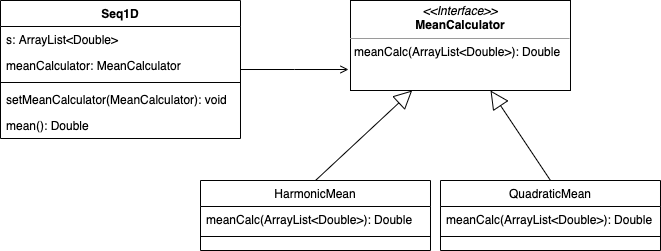
\includegraphics[scale=0.7]{Seq1D_Mean_Strategy_UML.png}
\end{center}
\caption{UML Class Diagram for Seq1D with Mean Function, using Strategy
  Pattern} \label{Fig_UML_Strategy}
\end{figure}

You will need to fill in the following blank files:
\texttt{MeanCalculator.java}, \texttt{HarmonicMean.java},
\texttt{QuadraticMean.java}, and \texttt{Seq1D.java}.  Two testing files are
also provided: \texttt{Expt.java} and \texttt{TestSeq1D.java}.  The file
\texttt{Expt.java} is pre-populated with some simple experiments to help you see
the interface in use, and do some initial testing.  You are free to add to this
file to experiment with your work, but the file itself isn't graded.  The
\texttt{TestSeq1D.java} is also not graded.  However, you may want to create
test cases to improve your confidence in your solution.  The stubs of the
necessary files are already available in your \texttt{src} folder.  The code
will automatically be imported into this document when the \texttt{tex} file is
compiled.  You should use the provided Makefile to test your code.  You will NOT
need to modify the Makefile.  The given Makefile will work for \texttt{make
  test}, without errors, from the initial state of your repo.  The \texttt{make
  expt} rule will also work, because all lines of code have been commented out.
Uncomment lines as you complete work on each part of the modules relevant to
those lines in \texttt{Expt.java} file.  As usual, the final test is whether the
code runs on mills.  You do not need to worry about doxygen comments.

Any exceptions in the specification have names identical to the expected Java
exceptions; your code should use exactly the exception names as given in the
spec.

Remember, your code needs to implement the given specification so that the
interface behaves as specified.  This does NOT mean that the local functions
need to all be implemented, or that the types used internally to the spec need
to be implemented exactly as given.  If you do implement any local functions,
please make them private.  The real type in the MIS should be implemented by
\texttt{Double} (capital D) in Java.

\wss{Complete Java code to match the following specification.}

%%%%%%%%%%%%%%%%%%%%%%%%%%%%%%%%%%

\newpage

\section* {Mean Calculator Interface Module}

\subsection*{Interface Module}

MeanCalculator

\subsection* {Uses}

None

\subsection* {Syntax}

\subsubsection* {Exported Constants}

None

\subsubsection* {Exported Types}

None 

\subsubsection* {Exported Access Programs}

\begin{tabular}{| l | l | l | p{5cm} |}
\hline
\textbf{Routine name} & \textbf{In} & \textbf{Out} & \textbf{Exceptions}\\
\hline
meanCalc & seq of $\mathbb{R}$ & $\mathbb{R}$ & ~\\
\hline
\end{tabular}

\subsubsection* {Considerations}

meanCalc calculates the mean (a real value) from a given sequence of reals.
The order of the entries in the sequence does not matter.

%%%%%%%%%%%%%%%%%%%%%%%%%%%%%%%%%%

\newpage

\section* {Harmonic Mean Calculation}

\subsection*{Template Module inherits MeanCalculator}

HarmonicMean

\subsection* {Uses}

MeanCalculator

\subsection* {Syntax}

\subsubsection* {Exported Constants}

None

\subsubsection* {Exported Types}

None 

\subsubsection* {Exported Access Programs}

\begin{tabular}{| l | l | l | p{5cm} |}
\hline
\textbf{Routine name} & \textbf{In} & \textbf{Out} & \textbf{Exceptions}\\
\hline
meanCalc & seq of $\mathbb{R}$ & $\mathbb{R}$ & ~\\
\hline
\end{tabular}

\subsection* {Semantics}

\subsubsection* {State Variables}

None

\subsubsection* {State Invariant}

None

\subsubsection* {Assumptions}

None

\subsubsection* {Access Routine Semantics}

meanCalc($v$)
\begin{itemize}
\item output: $\mathit{out} := \frac{|x|}{+(x: \mathbb{R} | x \in v : 1/x)}$
\item exception: none
\end{itemize}

%%%%%%%%%%%%%%%%%%%%%%%%%%%%%%%%%%

\newpage

\section* {Quadratic Mean Calculation}

\subsection*{Template Module inherits MeanCalculator}

QuadraticMean

\subsection* {Uses}

MeanCalculator

\subsection* {Syntax}

\subsubsection* {Exported Constants}

None

\subsubsection* {Exported Types}

None 

\subsubsection* {Exported Access Programs}

\begin{tabular}{| l | l | l | p{5cm} |}
\hline
\textbf{Routine name} & \textbf{In} & \textbf{Out} & \textbf{Exceptions}\\
\hline
meanCalc & seq of $\mathbb{R}$ & $\mathbb{R}$ & ~\\
\hline
\end{tabular}

\subsection* {Semantics}

\subsubsection* {State Variables}

None

\subsubsection* {State Invariant}

None

\subsubsection* {Assumptions}

None

\subsubsection* {Access Routine Semantics}

meanCalc($v$)
\begin{itemize}
\item output: $\mathit{out} := \sqrt{\frac{+(x: \mathbb{R} | x \in v : x^2)}{|x|}}$
\item exception: none
\end{itemize}

%%%%%%%%%%%%%%%%%%%%%%%%%%%%%%%%%%

\newpage

\section* {Seq1D Module}

\subsection* {Template Module}

Seq1D

\subsection* {Uses}

MeanCalculator

\subsection* {Syntax}

\subsubsection* {Exported Types}

Seq1D = ?

\subsubsection* {Exported Constants}

None

\subsubsection* {Exported Access Programs}

\begin{tabular}{| l | l | l | p{6cm} |}
\hline
\textbf{Routine name} & \textbf{In} & \textbf{Out} & \textbf{Exceptions}\\
\hline
new Seq1D & seq of $\mathbb{R}$, MeanCalculator & Seq1D & IllegalArgumentException\\
\hline
setMaxCalculator & MaxCalculator &  & \\
\hline
mean &  & $\mathbb{R}$ & \\
\hline

\end{tabular}

\subsection* {Semantics}

\subsubsection* {State Variables}

$s$: seq of $\mathbb{R}$\\
meanCalculator: MeanCalculator

\subsubsection* {State Invariant}

None

\subsubsection* {Assumptions}

\begin{itemize}
\item The Seq1D constructor is called for each object instance before any other
  access routine is called for that object.  The constructor can only be called
  once.  All real numbers provided to the constructor will be zero or positive.
\end{itemize}

\subsubsection* {Access Routine Semantics}

new Seq1D($x$, $m$):
\begin{itemize}
\item transition: $s, \text{meanCalculator} := x, m$
\item output: $\mathit{out} := \mathit{self}$
\item exception:
  $\mathit{exc} := (|x| = 0 \Rightarrow \mbox{IllegalArgumentException})$
\end{itemize}

\noindent setMeanCalculator($m$):
\begin{itemize}
\item transition: $\mbox{meanCalculator} := m$
\item exception: none
\end{itemize}

\noindent mean():
\begin{itemize}
\item output: $\mathit{out} := \mbox{meanCalculator.meanCalc}()$
\item exception: none
\end{itemize}

%%%%%%%%%%%%%%%%%%%%%%%%%%%%%%%%%%

\newpage

\subsection*{Code for MeanCalculator.java}

\noindent \lstinputlisting[language = Java]{./src/MeanCalculator.java}

\newpage

\subsection*{Code for HarmonicMean.java}

\noindent \lstinputlisting[language = Java]{./src/HarmonicMean.java}

\newpage

\subsection*{Code for QuadraticMean.java}

\noindent \lstinputlisting[language = Java]{./src/QuadraticMean.java}

\newpage

\subsection*{Code for Seq1D.java}

\noindent \lstinputlisting[language = Java]{./src/Seq1D.java}

%%%%%%%%%%%%%%%%%%%%%%%%%%%%%%%%%%

\end{document}